\documentclass{beamer}

\usetheme[department=compute]{DTU}

\usepackage[orientation=landscape,size=a1,scale=1.6,debug]{beamerposter}             

\usepackage{multicol} % This is so we can have multiple columns of text side-by-side
\columnsep=100pt % This is the amount of white space between the columns in the poster
\columnseprule=3pt % This is the thickness of the black line between the columns in the poster


\usepackage[T1]{fontenc}
\usepackage[utf8]{inputenc}
\usepackage{lmodern}
\usepackage[english]{babel}
%\usepackage{pgfplots}
%\pgfplotsset{compat=1.9}
%\usepackage{booktabs}
\usepackage{siunitx}


\title{Leverage based sampling for classification }
\author{Julian Kopka Larsen and Jesper Løve Hinrich}
\institute{DTU Compute}

\newcommand{\tabitem}{{\color{dtured}$\bullet$} }
\newenvironment{pblock}{\begin{minipage}[b]{\linewidth}
	\begin{block}}{\end{block} 	\end{minipage}}
\newcommand{\imblock}[1]{
\includegraphics[width=\linewidth]{#1}}

\begin{document}
\frame{
	\frametitle{Leverage based sampling for classification}
\begin{columns}[t]
    \begin{column}{.3\linewidth}



	

	\begin{pblock}{Introduction}
	We investigate a method for sampling the
	\end{pblock}
	
	\begin{pblock}{Motivation}
	The importance of sampling methods are initiated by very large datasets where it is not feasible to use all of the available data. This is illustrated by the rise in online access to online video data. These data contain many frames that are basically the same and therefore redundant. 
	\end{pblock}
	\begin{pblock}{What is leveraging}
	A sampling scheme based on covariances between datapoints. We define a probability distribution representing the "importance" of each datapoint and then sampling from that..  
	Shown by Ma et al. [1] to perform better than uniform on Least-Squares approximation on non-normal data.
	\end{pblock}
	    \end{column}
    \begin{column}{.3\linewidth}


	\begin{pblock}{Replicating their results}

	Shown by Ma et al. [1] to perform better than uniform on Least-Squares approximation on non-normal data.
	\end{pblock}
	
	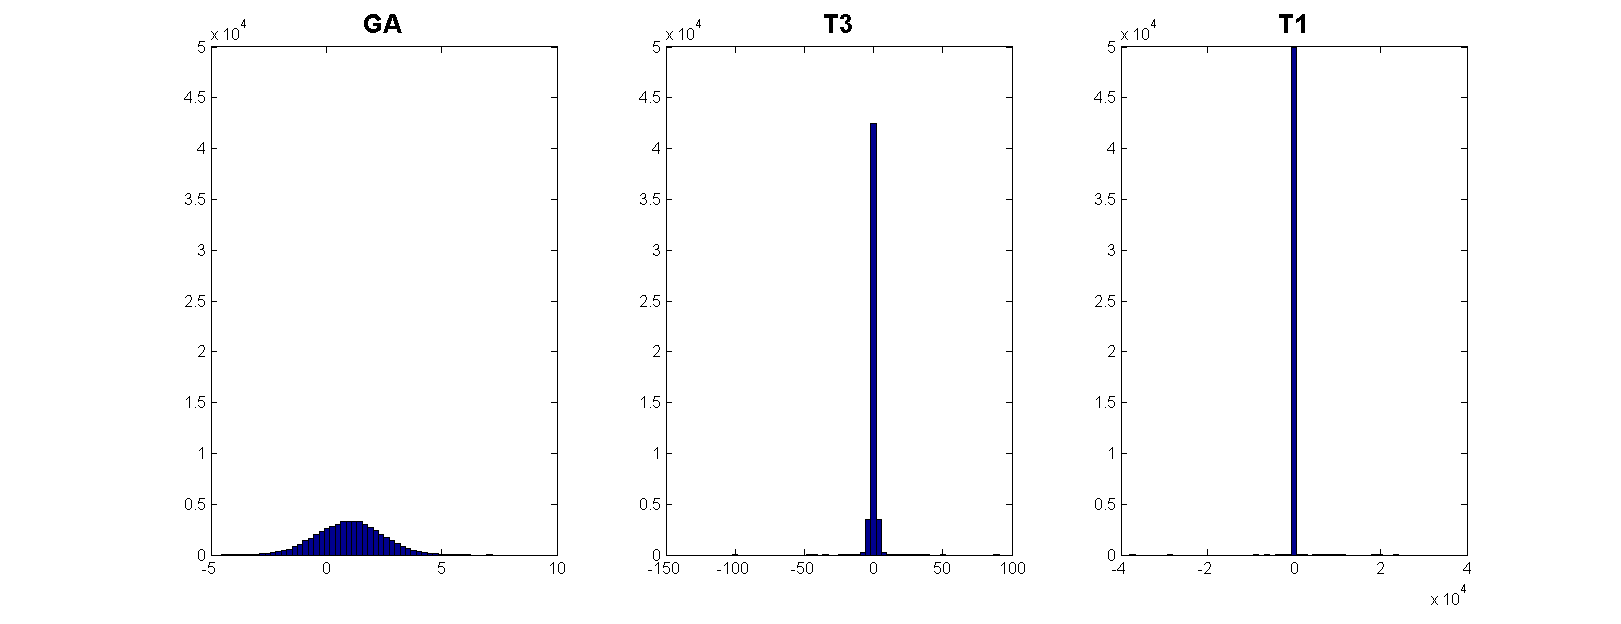
\includegraphics[width=\linewidth]{../Data_distributions.png}
	
	
    \end{column}
    \begin{column}{.3\linewidth}
    \end{column}
  \end{columns}
  }
\end{document}